\chapter{Implementierung}
\label{sec:Implementierung}

\section{Apache stanbol}
Um eine richtige Architektur des Systems auswählen zu können, fassen wir kurz die benötigte Komponenten zusammen:
\begin{itemize}
\item Eine Komponente für Training eines NER-Modells.
\item Eine Komponente für Extraktion von Entitäten aus Texten.
\item Ein Filter für ,,unpassende`` Entitäten.
\item Eine Komponente für Verlinkung von extrahierten Entitäten mit den Eigenschaften aus einer Wissendatenbank.
\item Eine API für Anreicherung von Suchergebnissen.
\end{itemize}

Damit alle aufgelistete Anforderungen im Rahmen dieser Arbeit implementiert werden könnten, muss ein Framework verwendet werden, das eine API für die Arbeit mit semantischen Daten ermöglicht. Im Rahmen dieser Arbeit wurde als solches Framework Apache Stanbol\footnote{\url{http://stanbol.apache.org/}} ausgewählt. Obwohl es andere Systeme, wie Alchemy API \footnote{\url{http://www.alchemyapi.com/}} gibt, die auch deutsche Sprache unterstützen, hat Stanbol gravierende Vorteile anderen Frameworks gegenüber:
\begin{itemize}
\item Die Quelltexte von Stanbol sind frei verfügbar, was die Entwicklung einer Erweiterung einfacher macht. Im Gegenteil dazu ist Alchemy API ein ,,Black Box`` - es gibt keine Möglichkeit, sich die in diesem Framework verwendete Algorithmen anzugucken oder die zu ändern, es gibt keine Möglichkeit, eigene Anpassungen durchzuführen.
\item Stanbol stellt dem Entwickler eine eingebettete REST-API zur Verfügung, was eine Ankopplung an Drittsysteme erleichtert.
\item Stanbol hat eine modulare Architektur, was bedeutet, dass die in dieser Arbeit benötigte Komponente sich genau so implementieren lassen, wie die beschrieben wurden, als Module.
\item Außerdem wird dem Entwickler eine interne Wissendatenbank zur Verfügung gestellt, was die Benutzung einer getrennter Software für die Implementierung der Verlinkung unnötig macht. 
\end{itemize}

\paragraph{}
Stanbol stellt dem Entwickler eine Plugin-API zur Verfügung, mit deren Hilfe neue Features wie Extraktion von Entitäten aus deutschen Texten leicht implementiert werden können. Die Liste von verfügbaren Modulen ist auf der Abbildung \ref{fig:komponenten} zusammengefasst.

\begin{figure}[ht]
\centering
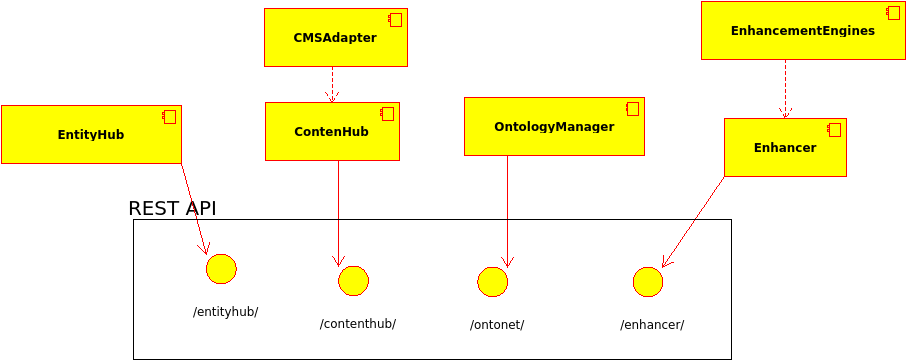
\includegraphics[width=0.6\textwidth]{Bilder/komponenten.png}
\caption{''Komponentendiagramm vom Stanbol''}
\label{fig:komponenten}
\end{figure}

\begin{itemize}
\item \textbf{EntityHub} ist die interne Datenbank, wo die Informationen über Entitäten gespeichert werden. Diese kann sowohl mithilfe von Java API als auch über eine REST-Schnittstelle für die Verlinkung benutzt werden. Als Datenquelle können sowohl ,,Referenced Sites`` (externe Datenquelle die sich auf anderen Maschinen befinden, und auf die EntityHub per Netzwerk zugreift) als auch lokale Indexes verwendet werden. Man kann EntityHub als eine Art von Aggregator betrachten, der mehrere Wissendatenbanke über eine einheitliche API zur Verfügung stellt. 
\item \textbf{Enhancer} und \textbf{EnhancementEngine} sind die Kernkomponenten von Stanbol, die für die Anreicherung von Texten mit Annotationen zuständig sind.
\item \textbf{OntologyManager} wird, wie sagt der Name, für die Verwaltung von Ontologien zuständig.
\item \textbf{ContentHub} wird für die Integration mit CMS gebraucht und stellt eine Datenbank für das \textit{Content} einer CMS zur Verfügung (nicht für die Entitäten!).
\end{itemize}
Im Rahmen dieser Arbeit werden nur Engines und EntityHub gebraucht, andere Module sind für die Extraktion von Entitäten irrelevant.

\paragraph{}
Die grundlegende Idee, die die Architektur von Stanbol prägt, heißt ,,Pipelining`` - ein Fließband, das mehrere Textverarbeitungsschritte miteinander verknüpft, und eine flexible Konfiguration von Kontentanreicherung ermöglicht. Jedes Element dieses Fließbandes wird ,,Engine`` genannt. Von dem Blickwinkel der Architektur wird jedes Engine als selbstständiges BlackBox implementiert, der am Eingang den Text, der angereichert werden soll, mit den von anderen Engines hinzugefügten Annotationen zusammen, bekommt, und am Ausgang neue Annotationen liefert. 

Die Engines werden in sogenannte Ketten zusammengebunden - der Ausgang von einem Engine wird mit dem Eingang von einem anderen Engine verbunden, und so wird eine virtuelle Kette gebaut. Das erste Element in dieser Kette bekommt dabei als Eingang den Text eines mithilfe von einer Suchmaschine gefundenen Snippets, und der Ausgang des letztes Element wird zu dem Benutzer geschickt. 

Auf der Abbildung \ref{fig:ENGINEPIPELINE} wird die Aufbau der in dieser Arbeit verwendeter Engine-Kette noch einmal grafisch dargestellt.
\begin{figure}[ht]
\centering
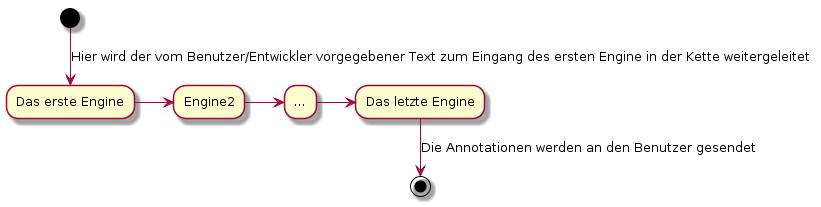
\includegraphics[width=\textwidth]{Bilder/enchancer.png}
\caption{''Graphische Darstellung des Anreicherungspipelines''}
\label{fig:ENGINEPIPELINE}
\end{figure}
Nachdem der Text, der angereichert werden soll, über REST API ausgelesen wurde, werden zuerst rohe Textdaten aus HTML extrahiert, was für Anreicherung von Webseiten notwendig ist. Falls die Daten aber schon im Plaintext gesendet wurden, wird dieser Schritt ignoriert. Danach muss die Sprache des Textes erkannt werden, anhand deren entschieden wird, ob der Text angereichert werden kann. Für die Erkennung der Sprache stellt Stanbol bereits ein Engine \footnote{\url{https://stanbol.apache.org/docs/trunk/components/enhancer/engines/langidengine.html}} zur Verfügung.

Falls die Sprache von der Kette unterstützt wird, werden die Sätze und Tokens extrahiert. Die Engines für Satz- und Tokenserkennung, die auch deutsche Sprache unterstützen, sind als Standardteil der API auch verfügbar.

Anschließend können aus dem Text, der vorberarbeitert wurde, Entitäten extrahiert werden. Nach den Extraktion-, Verlinkung- und Filterungsschritten wird der mit Annotationen angereicherte Text über REST-Schnittstelle zurückgegeben.

Als Entwickler muss man aber gleich beachten, dass die interne Implementierung von Ketten diese Architektur leider nicht anschaulich abbildet. Wie es auf der Abbildung \ref{fig:REALPIPELINE} zu sehen ist, gibt es intern kein Pipeline - stattdessen wird es für jeden Text, der angereichert werden soll, eine Instanz der Data-Klasse ,,ContentItem`` erzeugt, die zwischen allen Engines der Kette geteilt wird. Die Implementierung eines Engines hat technisch gesehen weder Ein- noch Ausgang, und benutzt diese Instanz von ,,ContentItem``, um die Informationen mit anderen Engines auszutauschen. Die Reihenfolge von Elementen in der Engine-Kette bestimmt deswegen eigentlich nicht, wie die Ein- und Ausgänge von Engines verbunden werden sollen, sondern die Reihenfolge, in der die ausgeführt werden müssen.

\begin{figure}[ht]
\centering
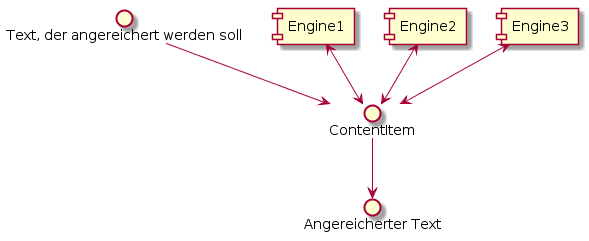
\includegraphics[width=\textwidth]{Bilder/realarch.png}
\caption{''Interne Implementierung einer Engine-Kette''}
\label{fig:REALPIPELINE}
\end{figure}
Der Nachteil solcher Architektur ist, dass mehrere Engines unter Umständen auf dieselbe Instanz von ,,ContentItem`` \textbf{gleichzeitig} zugreifen können, was bei Schreibzugriffen zur Beschädigung von Daten führen kann. Deswegen soll jedes Engine die Instanz von ,,ContentItem`` während des Schreibzugriffs sperren lassen.

Der Vorteil dieser Architektur besteht darin, dass bei Bedarf mehrere Engines parallel für den gleichen Content ausgeführt werden können. Dies kann z.B. dann nützlich sein, wenn es in mehreren Wissendatenbanken gleichzeitig nach den Informationen über eine Entität gesucht werden muss. Da das ,,ContentItem``-Objekt nur dann mit einem Lock gesperrt werden muss, wenn die Daten \textbf{geschrieben} werden, könnte \textbf{die Suche} in mehreren Wissendatenbanken gleichzeitig durchgeführt werden.

Um sicherstellen zu können, dass nur die Engines, die eine parallele Ausführung unterstützen, parallel gestartet werden, muss der Entwickler in der Konfiguration des Engines explizit eingeben, ob eine parallele Ausführung für das entwickelte Engine möglich ist.

\section{Extraktion von Entitäten} \label{sec:extraktimpl}
Da die Vorverarbeitungsschritte bereits als Teil von Stanbol implementiert sind, ist die Erkennung von Entitäten das erste Modul, das entwickelt werden muss. Die Schritte, die für die Entwicklung eines Engines unternommen werden müssen, lassen sich wie folgt definieren:
\begin{itemize}
\item Ein Engine wird als ein Objekt der Klasse ,,AbstractEnhancementEngine`` implementiert. 
\item Diese Klasse soll dem Framework folgende Methoden zur Verfügung stellen, die die Integration des Engines in eine Enginekette ermöglichen:
\begin{itemize}
\item Aktivierungsmethode, die ein mal beim Starten des Engines aufgerufen wird. Diese Methode soll das für das Engine benötigte Modell aus einer Datei laden (ein vortraniertes SVM, z.B.).
\item Die Methode, die für den angegebenen Text sagt, ob das Engine diesen Text anreichern kann. Dadurch wird sichergestellt, dass nur die Sprache, die ENgine tatsächlich versteht, bearbeitet wird.
\item Die Hauptmethode, die für den angegebenen Text Annotationen berechnet.
\end{itemize}
\item Die Ketten, die Engines miteinander verbinden, können sowohl während der Laufzeit als auch vor dem Kompilieren des Systems in einer Konfigurationsdatei definiert werden.
\end{itemize}

\subsection{StanfordNER} \label{subsec:stanfordner}
\paragraph{}
Die erste Anreicherungskette wurde auf Basis von StanfordNER\cite{Jenny/etal:07} aufgebaut. Dieses Framework implementiert CRF-Algorithmus und stellt ein Modell für die deutsche Sprache zur Verfügung\cite{faruqui10:_training}. Der Nachteil dieses Engines ist, dass es nur ein vortrainiertes Modell zur Verfügung gestellt wird - das Korpus selbst, auf deren Basis man eigenes Modell trainieren könnte, stehen nicht zur Verfügung. Der Vorteil dabei ist, dass es insgesamt zwei Modellen zur Verfügung stehen:

\begin{enumerate}
\item HGC - Huge German Corpus-generalized classifier - dieses Modell wurde auf Texten aus Zeitungen trainiert.
\item deWac - dieser Klassifikator wurde auf Texten aus Internet trainiert.
\end{enumerate}

Dieses Framework stellt außerdem die Möglichkeit zur Verknüpfung von mehreren Modellen miteinander zur Verfügung. Deswegen kann es im Rahmen dieser Arbeit neben dem Austesten von oben genannten Modellen auch ein kombiniertes Modell getestet werden - es ist möglich, dass ein kombiniertes Modell mehr Entitäten im Text finden könnte, andererseits steigt dabei die Wahrscheinlichkeit von False-Positive-Antworten.

Dieses Framework ist auch für Vorverarbeitung - Zerlegung des Textes in einzelne Sätze und Zerlegung von Sätzen in einzelne Tokens - verantwortlich. Deswegen sind für den auf Stanford-NER basierten Einsatz nur zwei Vorverarbeitung-Engines notwendig:
\begin{enumerate}
\item Tika-Engine für Extraktion von rohen Textdaten aus HTML.
\item Spracherkennungsmodul, mit deren Hilfe sichergestellt wird, dass die Analyse nur für deutsche Sprache gestartet wird.
\end{enumerate}

Die Klassendiagramm für dieses Engine ist auf der Abbildung \ref{fig:stanfclasses} zu sehen.

\begin{figure}[ht]
\centering
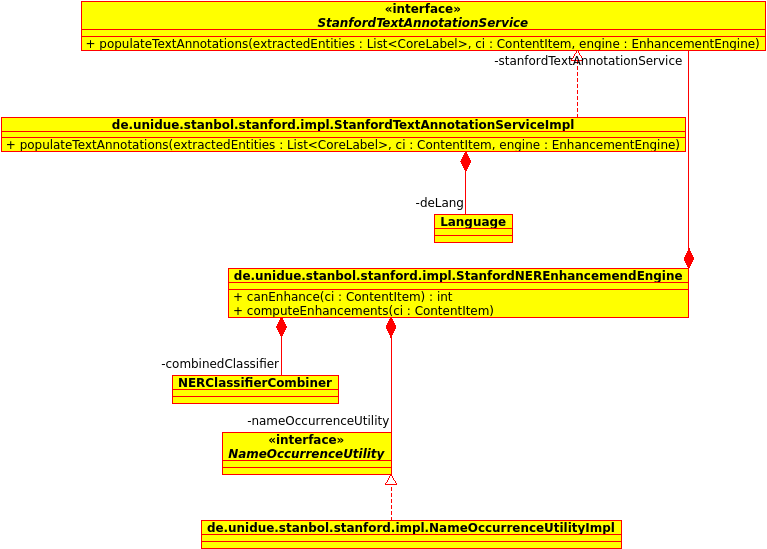
\includegraphics[width=\textwidth]{Bilder/stanford-classes.png}
\caption{''Klassendiagramm  des Stanford-Engines''}
\label{fig:stanfclasses}
\end{figure}
\begin{itemize}
\item Die Klasse \textit{StanfordNEREnhancementEngine} ist die Hauptklasse, die nach den Entitäten im Text sucht.
\item \textit{NERClassifierCombiner} ist die interne Klasse des StanfordNER-Frameworks und stellt die Schnittstelle zum Kombinieren von mehreren NER-Modellen zur Verfügung.
\item \textit{NameOccurenceUtility} ist eine Hilfsklasse, die die Daten zwischen StanfordNER- und Stanbol-Format umwandelt.
\item \textit{StanfordTextAnnotationService} ist ein Hilfsservice, das die vom Engine gefundene Entitäten	zum ,,ContentItem`` als Annotationen hinzufügt.
\end{itemize}

\subsection{OpenNLP}
%Beschreibung des OpenNLP-Einsatzes.
Das weitere Algorithmus, das im Rahmen dieser Arbeit verwendet wurde, ist MaximumEntropy. Es wurde als Teil von OpenNLP\footnote{\url{http://opennlp.apache.org/}}-API implementiert. OpenNLP ist ein quelltextoffenes Framework für maschinelle Sprachverarbeitung. Das Framework ist genau wie Stanbol modular aufgebaut, und stellt folgende Funktionalität zur Verfügung:

\begin{itemize}
\item Erkennung von Sätzen. Genau wie für die Extraktion von Entitäten wird für die Satzerkennung ein Maximum-Entropy-Modell verwendet, das vorher trainiert werden muss. Ein Modell für die deutsche Sprache, trainiert auf der Basis von TIGER-Korpus, der in nachfolgendem Kapitel beschrieben ist, ist aber bereits ein Teil des Frameworkes.
\item Zerlegung von Sätzen in Tokens:
\begin{itemize}
\item Die Zerlegung ohne Modell, nur anhand in dem Text vorhandenen Leerzeichen erfolgen. Diese Methode soll aber nicht verwendet werden, da die Fehlerwahrscheinlichkeit zu groß ist.
\item Es kann ein ME-Modell verwendet werden, um Tokens zu erkennen. Der Nachteil dieser Methode ist, dass das Modell zuerst trainiert werden soll, wozu ein Korpus gebraucht wird.
\end{itemize}
\item POS-Tagging - die Erkennung und Annotierung von Wortarten - während dieses Vorgangs wird jedem Token eine entsprechende Wortart zugeordnet.
\item Erkennung von Entitäten.
\end{itemize}

Der Vorteil dieses Engines ist, dass es schon als Teil von Stanbol dem Entwickler zur Verfügung stellt, und so muss nicht neu entwickelt werden. Allerdings müssen für die Extraktion von deutschsprachigen Entitäten die entsprechende ME-Modelle trainiert werden, worauf in der Sektion \ref{subsec:decor} angegangen wird.

Die Klassendiagramm für OpenNLP-Engine ist auf der Abbildung \ref{fig:onlpuml} definiert. Es werden insgesamt nur drei Klassen verwendet:
\begin{itemize}
\item Basisklasse \textit{NEREngineCore}, die die Extraktion von Entitäten mithilfe von ME-Algorithmus implementiert.
\item Die Klasse \textit{CustomNERModelEnhancementEngine}, die von der Basisklasse erbt, und für Behandlung von benutzerdefinierten Modellen zuständig ist.
\item Die Konfigurationsklasse \textit{NEREngineConfig}.
\end{itemize}

\begin{figure}[ht]
\centering
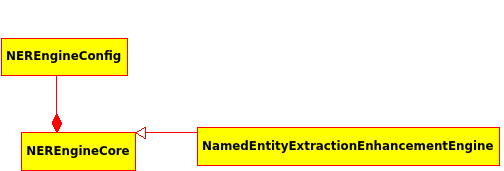
\includegraphics[width=\textwidth]{Bilder/onlp-classes.png}
\caption{''Klassendiagramm  des OpenNLP-Engines''}
\label{fig:onlpuml}
\end{figure}

\subsection{MITIE}
\paragraph{}
Der Einsatz, das implementiert werden soll, ist SVM-Algorithmus. Als Basis wurde für diese Arbeit MITIE\footnote{\url{https://github.com/mit-nlp/MITIE}}-Framework ausgewählt. MITIE steht für ,,MIT Information Extraction`` - ein Framework zur Extraktion von Entitäten und zur Erkennung von binären Relationen. Wie erwähnt, verwendet dieses Framework SVM als Basisalgorithmus für Erkennung von Entitäten, und soll deswegen auch bessere Ergebnisse als OpenNLP oder StanfordNER zeigen können.

\paragraph{Vor- und Nachteile}
\begin{itemize}
\item Vorteile des MITIE-Einsatzes:
\begin{enumerate}
\item Höhere Qualität der Extraktion, im Vergleich zu Maximum Entropy oder CRF.
\item Die Geschwindigkeit der Extraktion ist nicht viel kleiner, als die bei anderen Einsätzen.
\end{enumerate}
\item Nachteile des MITIE-Einsatzes:
\begin{enumerate}
\item Die Größe des Modells ist im Vergleich zu ME oder CRF-Modellen relativ hoch(323 Mb im Vergleich zu 3 Mb für ein OpenNLP-Modell)
\item Das Training eines SVM-Modells kann bis auf mehrere Tage dauern.
\item Ein rein technischer Nachteil - die MITIE-Implementierung ist in C++ geschrieben und ist außerdem nicht thread-sicher, was zu folgenden Einschränkungen führt:
\begin{enumerate}
\item Der Aufruf des Engines muss mit einem Lock gesichert werden, was die Geschwindigkeit bei mehreren gleichzeitigen Benutzer beeinträchtigt.
\item Jeder Fehler in dem Engine kann potentiell zum Absturz der ganzen JVM-Software führen.
\end{enumerate}
\end{enumerate}
\end{itemize}

Die Aufbau dieses Engines ähnelt sich der vom Stanford-NER-Engine, und kann auf der Abbildung \ref{fig:mitieclasses} betrachtet werden.

\begin{figure}[ht]
\centering
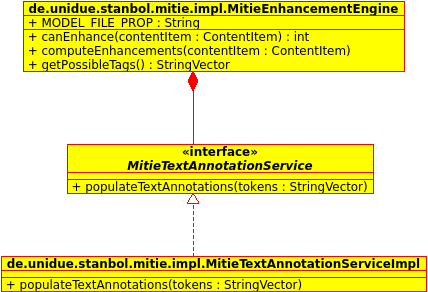
\includegraphics[width=\textwidth]{Bilder/mitie-classes.png}
\caption{''Klassendiagramm  des MITIE-Engines''}
\label{fig:mitieclasses}
\end{figure}
Die Klassen in diesem Engine spielen ähnliche Rollen, wie bei Stanford-NER mit einer gravierender Ausnahme: die Klasse \textit{NamedEntityExtractor}, die für die Extraktion von Entitäten verantwortlich ist, wird automatisch aus C++-Code erzeugt, und nicht manuell entwickelt.

\subsection{Deutcshe Korpora} \label{subsec:decor}
Nachdem die Engines, die nach Entitäten in Texten suchen sollen, entwickelt wurden, müssen die entsprechende NER-Modelle trainiert werden, wie es in der Sektion \ref{sec:trcorpora} beschrieben wurde. Und obwohl fällt dieser Schritt fürs auf Stanford-NER basierten Engine komplett aus, da dort ein vortrainiertes Modell verwendet wird, muss für weitere zwei Engines eigene Modelle trainiert werden.

Im Rahmen dieser Arbeit wurden zwei Trainingskoprora verwendet: von den Linguisten erzeugtes TIGER-Korpus und aus Basis von Wikipedia-Artikeln aufgebautes PIG-Korpus. Diese beide Korpora wurden aus folgenden Gründen ausgewählt:
\begin{itemize}
\item TIGER-Korpus wurde ausgewählt, da es das einzige deutschsprachige Korpus mit annotierten Entitäten ist, das frei verfügbar ist und das eine genügende Anzahl von Sätzen(50472 Sätzen) beinhaltet - das vom Sebastian Padó\cite{faruqui10:_training} zur Verfügung gestelltes Korpus ist zwar auch frei verfügbar, aber es beinhaltet nur 857 Sätzen, was fürs Training ungenügend ist.
\item Wikipedia wurde als Basis für automatisch aufgebautes Korpus ausgewählt, da die Dumps von Wikipedia frei verfügbar sind und eine große Anzahl von Daten (215841 Sätzen) beinhalten.
\end{itemize}

Für Training von Modellen für beide Engines (MITIE und OpenNLP) wird dasselbe Datenformat verwendet, das in der Auflistung \ref{lst:TIGEROPENBEISPIEL} beschrieben ist. Dadurch wird erreicht, dass der Code fürs Training von beiden Engines wiederverwendet werden kann.

\lstinputlisting[captionpos=b,label={lst:TIGEROPENBEISPIEL},caption={Ausschnitt aus einem Korpus im OpenNLP-Format.}]{Listings/tiger-opennlp.txt}

\subsubsection{TIGER Korpus}
\paragraph{}
TIGER-Korpus wurde von dem Institut für Maschinelle Sprachverarbeitung\cite{brants2004tiger} auf der Basis von Zeitungen aufgebaut, und beinhaltet 50474 Sätzen. Außer markierten Entitäten beinhaltet dieser Korpus auch die Informationen über POS (Part Of Speech - ob das Wort ein Verb oder ein Substantiv ist), Lemma (Infinitiv für Verben oder Nominativ Singular für Substantive) und andere Informationen über die annotierte Tokens, wie Kasus oder Genus. Der Ausschnitt des Korpuses findet man in der Auflistung \ref{lst:TIGERBEISPIEL}.

\lstinputlisting[captionpos=b,label={lst:TIGERBEISPIEL},caption={Ausschnitt aus dem TIGER-Korpus. Die Informationen, die in dieser Arbeit nicht gebraucht werden, wurden wegen Platzmangel weggelassen.}]{Listings/tiger-example.txt}
Jeder Satz ist dabei auf einer getrennter Zeile gespeichert, die Tokens werden mit Leerzeichen getrennt, und mithilfe von HTML-ähnlichen Tags werden die Entitäten markiert.

\paragraph{}
Der Korpus ist wie folgt aufgebaut:
\begin{itemize}
\item Die Sätze werden mit einer leeren Zeile getrennt.
\item Jeder Token und seine Annotationen werden in einer Zeile geschrieben. Die Spalten werden mit einem Leerzeichen getrennt.
\item Die erste Spalte beinhaltet ID des Tokens, die aus Nummer des Satzes und Nummer des Tokens innerhalb des Satzes besteht.
\item Die zweite Spalte ist der Token selbst, so wie er auch im Satz vorkommt.
\item In der dritten Spalte steht Lemma des Tokens.
\item Die vierte Spalte wird nicht verwendet.
\item Und die fünfte Spalte beinhaltet POS-Tag des Tokens. Falls dieser Tag den Typ \textit{NE} hat, ist das eine Entität.
\end{itemize}

Der Nachteil dieses Korpuses besteht darin, dass es zwischen verschiedenen Typen von Entitäten nicht unterschieden wird, und die alle den Typ \textit{NE} (NamedEntity) haben.

\paragraph{}
Die Logik, die für die Umwandlung von Tiger Korpuseinträgen in OpenNLP-Format verantwortlich ist, ist in der Auflistung \ref{lst:LOGICOFCONVERTER} zu sehen.
\lstinputlisting[captionpos=b,label={lst:LOGICOFCONVERTER},caption={Ausschnitt aus den Quelltexten des Konverters, der die Logik der Umwandlung beschreibt}]{Listings/tiger-to-onlp.java}
Es wird praktisch für jede ununterbrochene Reihenfolge von NE-Merkierungen ein OpenNLP-Tag erzeugt, und alle Wörter, die keine Entitäten sind, werden ohne Umwandlung kopiert.

\subsubsection{Wikipedia-basiertes Korpus}
\paragraph{}
Leider kann man nicht immer einen manuell aufgebauten Korpus verwenden, entweder aus Lizenz- oder Kostengründen. Viele Korpusse sind nur für Forschung frei verfügbar, was bedeutet, dass 
die auf keinen Fall in einem Geschäftsprojekt verwendet werden dürfen. Und einen eigenen Korpus aufzubauen ist auch nicht immer möglich, da dazu die Linguisten eingesetzt werden müssen, die nicht jede Firma zur Verfügung hat, und es kann Monaten dauern, bis man ein eigenes Korpus erstellt. Was könnte in diesem Fall unternommen werden?

\paragraph{}
Oliver Grisel\footnote{\url{http://www.nuxeo.com/blog/mining-wikipedia-with-hadoop-and-pig-for-natural-language-processing/}} hat einen interessanten Einsatz zur automatischer Aufbau von Korpus vorgeschlagen. Es wird vorgeschlagen, Wikipedia als Textbasis zu nehmen, und die interne Links, die auf andere Wikipediaseiten führen, sollen als  Entitäten markiert werden. Es soll anschließlich ein Korpus aufgebaut werden, auf dessen Basis ein NER-Modell trainiert werden kann. Da Wikipedia auch auf deutscher Sprache verfügbar ist, soll dieser Einsatz auch für Zwecke dieser Arbeit nützlich sein.

\paragraph{}
Um den Korpus aufzubauen, wird Apache Pig\footnote{\url{http://pig.apache.org/}} verwendet - ein Framework für Big-Data-Analyse, der eine Skript-Sprache und JavaAPI zur Verfügung stellt. Die Aufbau vom Korpus umfasst folgende Schritte:
\begin{enumerate}
\item Es wird Dump von Wikipediaartikeln heruntergeladen.
\item Es werden die Listen von Wikipedia-Links und Typen von Entitäten von DBpedia heruntergeladen. Diese Informationen braucht man später, um jeder Entität in dem erzeugten Korpus die richtige Entitätstyp zuordnen zu können.
\item Es werden Links auf interne Wikipedia-Artikeln aus Wikipedia-Dump extrahiert, mit der Positionsinformation zusammen.
\item Jeder Link wird mithilfe von DBpedia-Daten einen Entitätstyp zugeordnet.
\item Es wird ein Trainingskorpus im OpenNLP-Format erzeugt.
\end{enumerate}

\paragraph{} 
Für Korpusaufbau aus deutscher Wikipedia können im Prinzip die Scripts von Oliver Grisel genommen werden, die allerdings angepasst werden müssen:
\begin{itemize}
\item Es soll deutsche Dbpedia, und nicht englische verwendet werden.
\item Es soll deutsches Modell für Satzerkennung anstatt englisches eingesetzt werden.
\item Herunterladen von Wikipedia- und Dbpediadaten soll automatisiert werden.
\end{itemize}

Der Code, der für die Erzeugung eines Wikipedia-basierten Korpus verantwortlich ist, ist in der Auflistung \ref{app:pigcorpus} repräsentiert.

\paragraph{}
Aber welche Vor- und Nachteile hat automatische Erzeugung vom Korpus? Kann das trainierte Modell später auch tatsächlich für sinnvolle Entitätserkennung eingesetzt werden?
\begin{itemize}
\item Vorteile
\begin{itemize}
\item Die Erzeugung von Korpus braucht höchstens eine Stunde, im Vergleich zu manuell annotierten Korpora.
\item Es werden keine Fachleute gebraucht, um Korpus zu erzeugen.
\end{itemize}
\item Nachteile
\begin{itemize}
\item Nicht alle interne Links stellen eine Entität dar, und nicht alle Entitäten sind ein Link - als Folge ist die Qualität des Korpusses deutlich niedriger, als die von manuell aufgebauten.
\item Eine sehr niedrige Varianz - alle Wikipediaartikel sind mehr oder weniger in gleicher Sprache geschrieben, was bedeutet, dass wenn man dem trainierten Modell einen Text zeigt, der sich von einem durchschnittlichen Wikipedia-Artikel deutlich unterscheidet, werden da höchstwahrscheinlich keine Entitäten gefunden.
\end{itemize}
\end{itemize}

\subsection{Training von Modellen}
Sowohl für OpenNLP als auch für MITIE wird Training von Modellen außerhalb von Stanbol durchgeführt. Die Ergebnisse werden dabei in den binären Dateien serialisiert, und später von entsprechenden Engines innerhalb von Stanbol geladen. Der Grund, warum es so gemacht wurde, ist die Geschwindigkeit des Trainings - wie erwähnt, erfordert Training üblich viel größere Rechnerkapazitäten als die Verwendung von Modellen selbst, bei MITIE-Engine sind das mindestens 24 GB RAM, und Training dauert aber trotzdem bis auf eine Woche. Deswegen wurde Training auf getrennten Rechnern durchgeführt.

Die Implementierung von Training an sich selbst ist relativ einfach: 
\begin{enumerate}
\item Zuerst wird die vorab erzeugte OpenNLP-Training-Datei geladen.
\item Danach wird entweder OpenNLP- oder MITIE-API aufgerufen, um ein ME- oder SVM-Modell darauf zu trainieren.
\item Am Ende wird das erzeugte Modell serialisiert und in einer Datei gespeichert.
\end{enumerate}
Das Training von einem OpenNLP-Modell ist in der Auflistung \ref{app:trainonlp} und vom MITIE-Modell in der Auflistung \ref{app:trainmitie} beschrieben.

Beim Training vom MITIE-Modell mithilfe vom Wikipedia-Korpus(PIG) musste noch folgende Anpassung gemacht werden: ursprünglich musste das ganze Korpus (215841 Sätzen) fürs Training verwendet werden, allerdings konnte das Training auf einem Rechner mit 24 GB Arbeitsspeicher nicht abgeschlossen werden, deswegen wurden für MITIE zufällige Sätze aus dem PIG-Korpus ausgewählt (71947 Sätzen), und das Modell wurde auf dieser kleineren Korpusversion traianiert.

\section{Verlinkung und Dereferinzierung von annotierten Entitäten}
\paragraph{}
Nachdem die Entitätserkennung durchgeführt wurde, hat man die Informationen darüber, ob es Entitäten im Text gefunden wurden, die Position der Entität innerhalb des Satzes und optional die Klasse der Entität. Die Ontologie selbst, die Endbenutzer zu sehen braucht, fehlt allerdings noch. Es müssen noch zwei Schritte durchgeführt werden, bis die Informationen komplett sind - Verlinkung von gefundenen Entitäten mit der Entitäten in einer Wissendatenbank und die Dereferinzierung von Eigenschaften der Entität.

Als Datenquelle für die Verlinkung und Dereferinzierung wird in dieser Arbeit lokaler Index von deutscher DBpedia\cite{auer2007dbpedia} verwendet. DBPedia stellt eine Kopie von Wikipedia zur Verfügung, deren Daten als RDF-Graphen gespeichert werden, und auf die mithilfe von SPARQL zugegriffen werden kann.

Während der Verlinkung von Entitäten wird für jede erkannte Entität eine Suche nach dieser Entität in einer oder mehreren Wissendatenbanken durchgeführt. Um den Vorgang höchstmöglich zu beschleunigen, soll lokaler Wissendatenbankindex (EntityHub in Terminologie von Stanbol) eingesetzt werden. Dieser Index soll vorher aufgebaut werden, und zumindest die Namen der Entitäten beinhalten. Für spätere Schritte ist aber empfehlenswert, auch diverse Eigenschaften von Entitäten zum Index hinzuzufügen, damit Dereferinzierungschritt auch so schnell wie möglich ausgeführt wird. Es muss aber beachtet werden, dass Index von realen Wissendatenbanken wie DBpedia mehr als 20 Gigabytes auf Festplattenspeicher verbrauchen kann, und die Aufbau kann mehrere Tagen in Anspruch nehmen.

Für die Verlinkung von Entitäten wird Engine ,,EntityLinkingEngine`` verwendet, dessen Aufbau auf der Abbildung \ref{fig:linking} beschrieben ist.

\begin{figure}[ht]
\centering
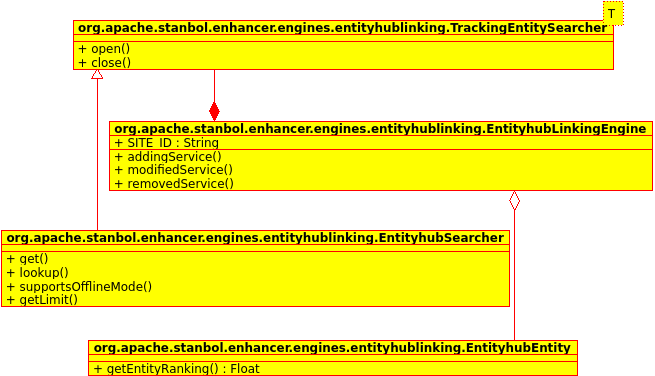
\includegraphics[width=\textwidth]{Bilder/classes-linking.png}
\caption{''UML-Klassendiagramm für EntityLinkingEngine''}
\label{fig:linking}
\end{figure}
\begin{itemize}
\item Die Klasse \textit{EntityHubSearcher}, die Interface \textit{TrackingEntitySearcher} implementiert, ist für die Suche in der Wissendatenbank zuständig.
\item Die Klasse \textit{EntityHubEntity} stellt eine Entität und ihre Eigenschaften dar. Das Parameter ,,entityRank`` zeigt, wie wichtig die Entität ist, was für die Rausfilterung von ,,unpassenden`` Entitäten helfen könnte.
\item \textit{EntityhubLinkingEngine} ist die Hauptklasse, die die Informationen über extrahierte Entitäten verlinkt.
\end{itemize}

Bei der Verlinkung von Entitäten kommt es oft vor, dass die Entitäten, die gefunden wurden, eigentlich nur Verlinkungen auf andere Entitäten, und keine selbstständige Objekten sind - z.B. die Entität ,,CDU`` ist nur ein Link auf ,,Christlich Demokratische Union Deutschlands`` ist. Solche Entitäten werden während der Verlinkung anhand der Eigenschaft ,,dbo:wikiPageWikiLink`` erkannt, und anstatt dieser Zwischenentität wird als Ergebnis der Verlinkung die referenzierende Entität verwendet.

Um die für den Benutzer relevante Informationen (Eigenschaften von Entitäten) zur Verfügung stellen zu können, müssen diese Eigenschaften aus der Datenbank geladen werden. Dazu könnte man auch direkt auf die entsprechende Schnittstelle zugreifen (http://de.dbpedia.org/resource/ für DBpedia, zum Beispiel), so ein Vorgehen würde aber zeitaufwändig und ineffektiv sein. Deswegen soll auch für die Dereferinzierung EntityHub eingesetzt werden. Für diesen Zweck wird Engine \textit{EntityhubDereferenceEngine} eingesetzt, der für jede im Verlinkungsschritt gefundene Entität alle für den Link verfügbare Eigenschaften zu dem Anreicherungsergebnis hinzufügt. Die Klassendiagramm für dieses Engine ist auf der Abbildung \ref{fig:deref} zu sehen. 

\begin{figure}[ht]
\centering
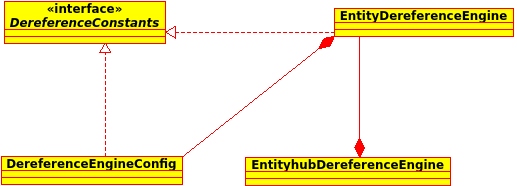
\includegraphics[width=\textwidth]{Bilder/deref-uml.png}
\caption{''UML-Klassendiagramm für EntityhubDereferenceEngine''}
\label{fig:deref}
\end{figure}
Theoretisch können hier auch SQL-Datenbanke für die Dereferenzierung verwendet werden - es muss nur eine eigene Klasse, die vor dem Interface \textit{ENtityDereferenceEngine} erbt, implementiert werden, aber wegen der möglichen Problemen, die in der Einleitung (\ref{sec:wiss}) beschrieben wurden, wäre es nicht empfohlen.

\section{Rausfilterung von für den Benutzer irrelevanten Entitäten}
Wie in der Aufgabenstellung (\ref{sec:Aufgabenstellung}) gesagt wurde, müssen nur relevante Entitäten dem Benutzer angezeigt werden, damit der Benutzer sich nicht verwirrend fühlt. Die beste Lösung dieses Problems wäre eventuell eine semantische Analyse der Benutzeranfrage, und ein Matching von Entitäten mit den Ergebnissen solcher Analyse, aber wegen Zeitmangel und einem zu großen Aufwand, der außer Rahmen dieser Masterarbeit stünde, konnte diese Lösung nicht implementiert werden. Statdessen werden folgende Gewichte verwendet, um zu entscheiden, ob eine Entität wichtig genug ist:
\begin{itemize}
\item Das Gewicht der Entität innerhalb des EntityHubs verwendet, das anhand von Anzahl der Wikipedia-Links, die auf die Entität zeigen, festgesetzt wird.
\item Das ,,Sicherheitwert`` (Confidence) des Extraktion-Engines bezüglich der Entität - jedes Engine fügt dieses Wert hinzu, um dem Entwickler mitzuteilen, wie ,,sicher`` diese Entität sein soll.
\end{itemize}

Das Engine, das diesen Filter implementiert, besteht nur aus einer Klasse, deren Funktionsweise auf der Abbildung \ref{fig:seqfilter} dargestellt ist.

\begin{figure}[ht]
\centering
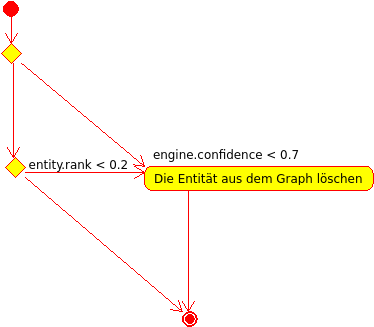
\includegraphics[width=0.8\textwidth]{Bilder/seqfilter.png}
\caption{''Funktionsweise des Filters''}
\label{fig:seqfilter}
\end{figure}
Die Schwellwerte für beide Filter (0.7 für Confidence und 0.2 für den Rank) wurden nach manuellem Austesten von Engines anhand persönlichen Erfahrungen des Entwicklers ausgewählt.

\section{API f{\"{u}}r Anreicherung von Suchergebnissen}
\paragraph{}
Um dem Endentwickler die Anreicherung von Suchergebnissen so einfach wie möglich zu machen, wurde eine API entwickelt, die direkt an ein beliebiges Java-Projekt als eine Bibliothek angebunden werden kann. Diese Bibliothek wird auch später in der Evaluierung verwendet. Es wurde eine Abstraktionsschicht hinzugefügt, die die Aufrufe der REST-Schnittstelle von Stanbol hinter der Klientklasse verbirgt. Der Entwickler soll nur die Liste von Suchsnippets an API übergeben, für die Verbindungaufbau zum Stanbol und Parsing der Antwort des Servers ist API verantwortlich. Die Beschreibung der API-Schnittstelle, die für den Entwickler sichtbar ist, findet man in der Auflistung \ref{lst:APISCHNITSTELLE}. 

Als Eingabedaten übergibt man die Liste von URLs gefundenen Webseiten mit dazugehörigen Texten von Snippets zusammen, und als Ausgabe bekommt man für jede URL die Liste von gefundenen Entitäten. Da in Rahmen dieser Arbeit mehr verschiedenen Engineketten implementiert wurden, muss der Name der erwünschten Kette miteingegeben werden.

Die API wurde außerdem so entworfen, dass bei Bedarf nicht nur Stanbol, sondern jedes beliebiges System als Backend verwendet werden kann - für jedes neues Backend muss nur die Klasse ,,EnhancementClient`` abgeleitet werden, und in der abgeleiteten Klasse die Schnitstelle zum neuen System implementiert werden. Gegebenfalls sollen auch neue Konverter geschrieben werden, falls Backend keine RDF-Daten liefert, und eigenes Datenformat verwendet.

Eine UML-Klassendiagramm für die Stanbol-API ist auf der Abbildung \ref{fig:apiuml} zu sehen. Es soll beachtet werden, dass die Schnitstelle zur Suchmaschine absichtlich außer Acht gelassen wurde - um die API so generisch wie möglich zu gestalten, wird die Anbindung an Suchmaschine dem Entwickler, der die API verwendet, überlassen. 

\begin{figure}[ht]
\centering
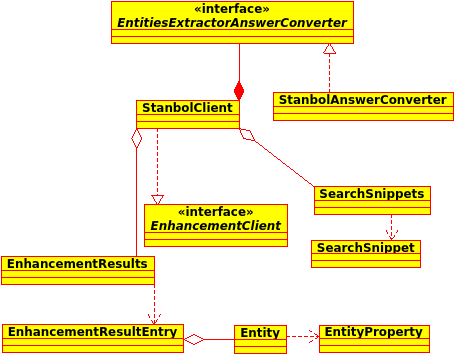
\includegraphics[width=\textwidth]{Bilder/apiuml.png}
\caption{''Struktur der Stanbol-API''}
\label{fig:apiuml}
\end{figure}
\begin{itemize}
\item Die Klasse \textit{StanbolClient} implementiert das Interface \textit{EnhancementClient}, und spielt die Rolle der Hauptklasse für die Konversation mit Stanbol.
\item \textit{StanbolAnswerConverter} umwandelt die Antwort des Stanbol-Servers (RDF) in das interne API-Format:
\begin{itemize}
\item Die Klasse \textit{EnhancementResults}, die als ein Container für gefundene Entitäten dient.
\item Die Klasse \textit{EnhancementResultEntry}, die die  Ergebnisse der Extraktion für eine bestimmte Webseite zusammenfasst.
\item \textit{Entity}, die eine Entität mit den Parametern zusammen (als eine Liste von \textit{EntityProperty}) darstellt.
\end{itemize}
\item Die Klassen \textit{SearchSnippets} und \textit{SearchSnippet} werden für die Zwischenspeicherung von den Snippets und URLs, die eine Suchmaschine geliefert hat, verwendet. Die Schnittstelle zu der Suchmaschine wird von dem Entwickler implementiert.
\end{itemize}